\documentclass{VUMIFPSbakalaurinis}
\usepackage{algorithmicx}
\usepackage{algorithm}
\usepackage{algpseudocode}
\usepackage{amsfonts}
\usepackage{amsmath}
\usepackage{bm}
\usepackage{caption}
\usepackage{color}
\usepackage{float}
\usepackage{graphicx}
\usepackage{listings}
\usepackage{subfig}
\usepackage{url}
\usepackage{wrapfig}
\usepackage[table,xcdraw]{xcolor}
\usepackage[backend=biber]{biblatex}
\usepackage{enumitem}\setlist{nosep}
\usepackage{listings}

% Titulinio aprašas
\university{Vilniaus universitetas}
\faculty{Informatikos Institutas}
\department{Programų sistemų katedra}
%\papertype{Bakalauro darbas}
\papertype{Bakalauro darbas}
\title{Anomalijų aptikimas Interneto Prieigos Stebėsenos Sistemos įrašuose}
\titleineng{Detection of anomalies in Internet Access Monitoring System data}
\author{Jokūbas Rusakevičius}
\supervisor{asist. dr. Vytautas Valaitis}
\reviewer{j. asist. Linas Petkevičius}
\date{Vilnius – \the\year}

% Nustatymai
\setmainfont{Palemonas}  
\bibliography{bibliografija}

\begin{document}
\maketitle

\setcounter{page}{2}

%% Padėkų skyrius
%\sectionnonumnocontent{}
%\vspace{7cm}
%\begin{center}
%	Padėkos asmenims ir/ar organizacijoms
%\end{center}

\sectionnonumnocontent{Santrauka}
Glaustai aprašomas darbo turinys: pristatoma nagrinėta problema ir padarytos
išvados. Santraukos apimtis ne didesnė nei 0,5 puslapio. Santraukų gale
nurodomi darbo raktiniai žodžiai. 
% Nurodomi iki 5 svarbiausių temos raktinių žodžių (terminų).
% Vienas terminas gali susidėti iš kelių žodžių.
\raktiniaizodziai{raktinis žodis 1, raktinis žodis 2, raktinis žodis 3, raktinis žodis 4, raktinis žodis 5}   

\sectionnonumnocontent{Summary}
Santrauka anglų kalba. Santraukos apimtis ne didesnė nei 0,5 puslapio.
\keywords{keyword 1, keyword 2, keyword 3, keyword 4, keyword 5}

\tableofcontents

\sectionnonum{Įvadas}
Įvade nurodomas darbo tikslas ir uždaviniai, kuriais bus įgyvendinamas tikslas,
aprašomas temos aktualumas, apibrėžiamas tiriamasis objektas akcentuojant
neapibrėžtumą, kuris bus išspręstas darbe, aptariamos teorinės darbo prielaidos
bei metodika, apibūdinami su tema susiję literatūros ar kitokie šaltiniai,
temos analizės tvarka, darbo atlikimo aplinkybės, pateikiama žinių apie
naudojamus instrumentus (programas ir kt., jei darbe yra eksperimentinė dalis).
Darbo įvadas neturi būti dėstymo santrauka. Įvado apimtis 2–4 puslapiai.

\subsectionnonum{Problematika}
TODO

\section{Medžiagos darbo tema dėstymo skyriai}
Medžiagos darbo tema dėstymo skyriuose išsamiai pateikiamos nagrinėjamos temos
detalės: pradiniai duomenys, jų analizės ir apdorojimo metodai, sprendimų
įgyvendinimas, gautų rezultatų apibendrinimas.

Medžiaga turi būti dėstoma aiškiai, pateikiant argumentus. Tekste dėstomas
trečiuoju asmeniu, t.y. rašoma ne „aš manau“, bet „autorius mano“, „autoriaus
nuomone“. Reikėtų vengti informacijos nesuteikiančių frazių, pvz., „...kaip jau
buvo minėta...“, „...kaip visiems žinoma...“ ir pan., vengti grožinės
literatūros ar publicistinio stiliaus, gausių metaforų ar panašių meninės
išraiškos priemonių.

Skyriai gali turėti poskyrius ir smulkesnes sudėtines dalis, kaip punktus ir
papunkčius.

\subsection{Poskyris}
Citavimo pavyzdžiai: cituojamas vienas šaltinis \cite{PvzStraipsnLt}; cituojami
keli šaltiniai \cite{PvzStraipsnEn, PvzKonfLt, PvzKonfEn, PvzKnygLt, PvzKnygEn,
	PvzElPubLt, PvzElPubEn, PvzMagistrLt, PvzPhdEn}.

\section{Duomenų analizės eksperimentas naudojant „MacroBase SQL“ modulį}

\subsection{Duomenų rinkinys}
Šiame skyriuje aprašyti eksperimentui pritaikyti IPSS duomenų rinkiniai.

\subsubsection{Eksperimentui pritaikyti duomenys}
Eksperimentui buvo naudojami Lietuvos Respublikos ryšių reguliavimo tarnybos administruojamos Interneto prieigos stebėsenos sistemos (IPSS) atliekami belaidės interneto prieigos duomenų perdavimo spartos kontrolinių matavimų 2014–2018 metų rezultatai. Matavimai atlikti operatorių UAB „Bitė Lietuva“, AB „Telia Lietuva“, UAB „TELE2“ ir AB Lietuvos radijo ir televizijos centro (LRTC) judriojo ryšio tinkluose visoje Lietuvos teritorijoje. Matavimų paskirtis yra stebėti ir įvertinti teikiamų interneto prieigos paslaugų kokybę, kaip to reikalauja Europos Sąjungos direktyvos, taip pat supažindinti visuomenę su tokių matavimų rezultatais. Įrašai pateikiami CSV formato failais. Iš viso gauti 3 failai skirti trims skirtingoms technologijoms: 3G, LTRE ir WiMAX. Viename CSV faile priklausomai nuo failui priskirtos technologijos buvo apytiksliai 136000, 157000 ir 18000 įrašų eilučių, vidutiniškai 104000. Vieno failo dydis vidutiniškai 8,5MB.

\subsubsubsection{Duomenų aprašymas}
Kiekvienas IPSS įrašų failas prasideda antraštės (angl. \textit{header}) eilute, kuri susideda iš faile saugomų įrašų sąrašo laukų (angl. \textit{fields}) pavadinimų. IPSS įrašų sarašų laukai ir jų paaiškinimas:

\begin{itemize}
	\item \textbf{Bendri visiems failams laukai:}
		\subitem \textbf{Data ir laikas} – matavimo įrašo fiksavimo data ir laikas, užrašoma „yyyy-MM-dd hh:mm:ss“ formatu.
		\subitem \textbf{Platuma} – matavimo įrašo fiksavimo koordinačių platuma užrašoma dešimtainiais laipsniais (angl. \textit{decimal degrees}).
		\subitem \textbf{Ilguma} – matavimo įrašo fiksavimo koordinačių ilguma užrašoma dešimtainiais laipsniais (angl. \textit{decimal degrees}).
		\subitem \textbf{Operatorius} – matavimo įrašo operatoriaus skaitinis kodas arba pavadinimas (vieno iš jau minėtų operatorių: „Bitė Lietuva“, „Telia Lietuva“, „TELE2“ ir LRTC).
		\subitem \textbf{RSSI} – signalo stiprumo indikatorius (angl. \textit{received signal strength indicator}).
		\subitem \textbf{Sparta kbit/s} – sveikuoju skaičiumi nurodomas užfiksuotas matavimo greitis kilobitais per sekundę.
	\item \textbf{3G failui išskirtiniai laukai:}
		\subitem \textbf{Celės id} – matavimą atlikusio įrenginio identifikacijos kodas.
		\subitem \textbf{Ryšio tinklas} – nurodo matuojamo ryšio tinklą (visi įrašai šiame faile ryšio tinklo lauke turi reikšmę „3G“).
		\subitem \textbf{3G ryšio technologija} – nurodo matavimo metu naudotą ryšio technologiją (vieną iš: „DC-HSPA+“, „HSDPA“, „HSPA“, „HSPA+“, „HSUPA“ arba „WCDMA“).
	\item \textbf{LTE failui išskirtiniai laukai:}
		\subitem \textbf{Celės id} – matavimą atlikusio įrenginio identifikacijos kodas.
		\subitem \textbf{RSRP} – angl. \textit{reference signals received power} panašiai kaip RSSI signalo stiprumo identifikatorius LTE tinklams.
		\subitem \textbf{RSRQ} – angl. \textit{reference signals received quality} signalo kokybės laukas (šiame dokumente šis laukas reikšmės neturi – „NULL“)).
		\subitem \textbf{SINR} – signalo ir trukdžių bei triukšmo santykis (angl. \textit{signal-to-interference-plus-noise ratio}) (šiame dokumente šis laukas reikšmės neturi – „NULL“)).
		\subitem \textbf{Ryšio tinklas} – nurodo matuojamo ryšio tinklą (visi įrašai šiame faile ryšio tinklo lauke turi reikšmę „LTE“).
	\item \textbf{WiMAX failui išskirtiniai laukai:}
		\subitem \textbf{Bazinės stoties id} – matavimą atlikusios stotelės MAC adresas.
		\subitem \textbf{CINR} – trikdžių ir triukšmo santykis (angl. \textit{carrier to interference-plus-noise ratio}).
		\subitem \textbf{Ryšio technologija} – nurodo matuojamo ryšio tinklą (visi įrašai šiame faile ryšio technologijos lauke turi reikšmę „WIMAX“).
\end{itemize}


\begin{figure}[H]
	\centering
	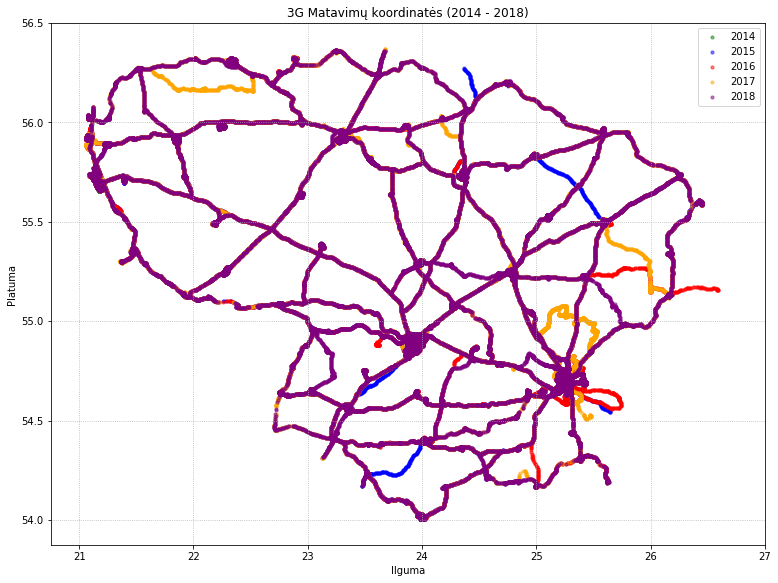
\includegraphics[scale=0.5]{img/3G-0}
	\caption{3G Matavimai 2014–2018 metais.}
	\label{img:3G-0}
\end{figure}
\begin{figure}[H]
	\centering
	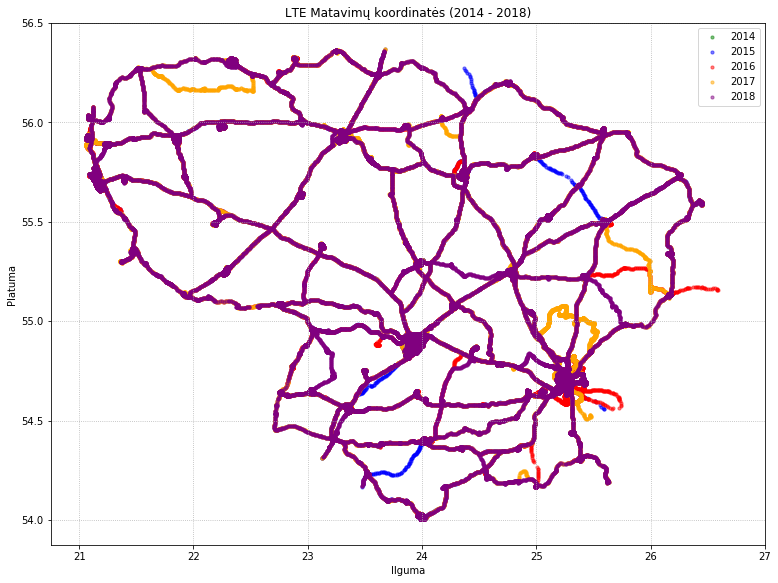
\includegraphics[scale=0.5]{img/LTE-0}
	\caption{LTE Matavimai 2014–2018 metais.}
	\label{img:LTE-0}
\end{figure}
\begin{figure}[H]
	\centering
	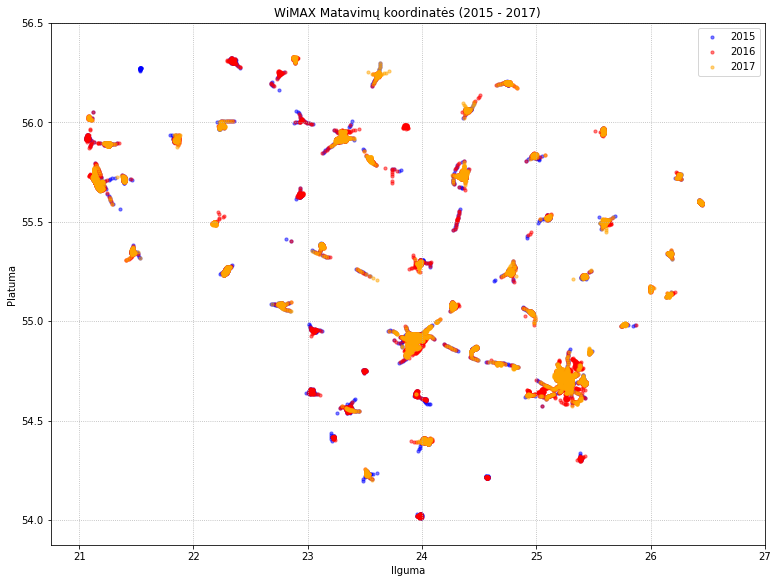
\includegraphics[scale=0.5]{img/WiMAX-0}
	\caption{WiMAX Matavimai 2015–2017 metais.}
	\label{img:WiMAX-0}
\end{figure}
Aiškiau išskirtus įrašų koordinačių duomenis galima rasti Priede \ref{coordpav}.


\subsubsubsection{Duomenų paruošimas}
Eksperimentui atlikti buvo atrinkti laukai, kurie turi reikšmes visose įrašų sąrašo eilutėse bei taip pat buvo atmesti pasikartojančios informacijos laukai (ryšio tinklo ir ryšio technologijos laukai, kurie nurodo, koks tinklo tipas iš trijų tiriamųjų yra naudojamas faile). Taip pat buvo nuspręsta datos ir laiko lauką pakeisti tik metų lauku. Taigi, 3G tinklui atrinkti šie pradiniai laukai: metai, ilguma, platuma, operatorius, celės id, rssi, 3G ryšio technologija ir sparta; iš LTE duomenų atrinkti laukai: metai, ilguma, platuma, operatorius, celės id, rssi, rsrp, sparta; iš WiMAX duomenų atrinkti laukai: metai, ilguma, platuma, operatorius, bazinės stoties id, rssi, cirn, sparta.\par
Eksperimentui atlikti buvo reikalingas CSV formato failai, kuriuose nebūtų lietuviškų raidžių ir būtų naudojami vieno žodžio arba vienos simbolių eilutės antraštės pavadinimai (pavyzdžiui, tarpai gali būti pakeičiami „\_“ simboliu), todėl buvo realizuoti „Python“ skriptas, kuris nuskaito duotųjų duomenų CSV failus ir juos apdorojus, grąžina naujus CSV failus. Skriptas kurtas ir leistas „Jupyter Notebook“ aplinkoje. Skripte galima pasirinkti kelią iki duotųjų CSV failų ir kelią iki naujai sukuriamų CSV failų. Šis skriptas skirtas pervadinti antraštes, atskirti metus ir atrinkti nereikalingus laukus. Skriptai atlieka šiuos veiksmus 3 kartus kiekvienai ryšio technologijai (3G, LTE, WiMAX) (Priedas \ref{script1}):
\begin{enumerate}
	\item Nuskaito CSV įrašų failą pateiktą nurodytu keliu.
	\item Sukuria naują CSV failą nurodytų keliu ir pavadinimu.
	\item Įrašo į naujai sukurtą CSV failą, naują antraštę, su naujais angliškais vieno žodžio (simbolių eilutės) pavadinimais.
	\item Vykdo ciklą, kuris skaitant po vieną eilutę iš pradinio failo įrašo tik reikalingus duomenis į naują failą bei iš datos ir laiko paima tik metus. Taip pat kiekviena eilutė yra skaičiuojama.
	\item Išvedamas galutinis eilučių skaičius.
\end{enumerate}
Atrinkus duomenis iš pradinių duomenų buvo sukurtas antras skriptas skirtas išgauti daugiau informacijos iš koordinačių. Kadangi ilgumos ir platumos laukai yra realiosios reikšmės, jomis yra nepatogu naudotis. Tam buvo sukurtas dar vienas skriptas, kuris suapvalina koordinačių laukus iki pasirinkto skaičiaus po kableliu taip sumažinant unikalių reikšmių kiekį. Šios reikšmės buvo pridėtos į joms sukurtus naujus laukus. Papildomai originalios koordinačių reikšmės buvo panaudotos išgauti kiekvieno koordinačių taško aukštį virš jūros lygio. Ši bei suapvalinta iki dešimčių metrų reikšmės buvo pridėtos į papildomus joms sukurtus laukus. Taigi naujas „Python“ skriptas nuskaito prieš tai sukurtus CSV failus, gauna aukščio virš jūros lygio reikšmes, suapvalina koordinačių bei aukščio reikšmes ir sukuria naujus CSV failus pasirinktu adresu. Skriptai atlieka šiuos veiksmus 3 kartus kiekvienai ryšio technologijai (3G, LTE, WiMAX) (Priedas \ref{script2}):
\begin{enumerate}
	\item Nuskaito CSV įrašų failą pateiktą nurodytu keliu.
	\item Iš nuskaitytų duomenų atskiriama antraštė nuo įrašų.
	\item Iš antraštės surandami metų, platumos ir ilgumos laukų indeksai.
	\item Pasinaudojus gautais indeksais, sukuriami visų ilgumos ir platumos reikšmių masyvai.
	\item Vykdomas ciklas, kuris visus įrašus padalina į pasirinkto žingsnio dydžio dalis.
	\item Vykdomas ciklas cikle, kuris visas ilgumos ir platumos reikšmes sujungia į „string“ tipo kintamuosius, kuriuose ilguma ir platuma yra atskirtos kableliu „,“.
	\item Kiekvienam žingsniui, iš platumos ir ilgumos bendrų kintamųjų sukuriamas vienas „string“ kintamasis, kur kiekvienas bendras koordinačių kintamasis yra atskirtas vertikaliu brūkšniu „|“.
	\item Vykdomas ciklas, kuris kiekvienai žingsnio koordinačių kiekio „string“ kintamajam sukuria URL užklausą „Jawg.io“ API, kuri susideda iš koordinačių kintamojo, pagrindinio URL ir vartotojo prieigos žymės (angl. \textit{access token}).
	\item Kiekvienam žingsniui yra siunčiama HTTP užklausa, kuri grąžina JSON duomenų struktūrą su koordinatėmis ir jų aukščiais virš jūros lygio.
	\item Iš JSON duomenų struktūros atskiriamos aukščio virš jūros lygio reikšmės ir jos yra patalpinamos į masyvą atitinkamu indeksu.
	\item Vykdomas ciklas, kuris kiekvienam nuskaitytam įrašui sukuria nauja įrašą su suapvalintomis iki pasirinkto skaičiaus po kablelio reikšmėmis bei aukščio virš jūros lygio ir suapvalinta iki dešimčių aukščio virš jūros lygio reikšmėmis. Šie įrašai sujungiami su atitinkamais įrašais ir sukuriamas naujas masyvas su šiais įrašais.
	\item Sukuriamas naujas CSV failas nurodytu keliu ir pavadinimu.
	\item Įrašoma nauja antraštė su papildytais pavadinimais.
	\item Vykdomas ciklas, kuris kiekvieną naujai papildytą įrašą įveda į naują CSV failą.
\end{enumerate}
Eksperimentui atlikti buvo nuskaityti ir apdoroti apie 300000 įrašų, vidutiniškai 100000 per failą.
TODO: pridėti citatą
\subsection{Eksperimento aplinkos paruošimas}

\subsection{Eksperimento vykdymo eiga}

\subsubsection{Konfiguracija}









\sectionnonum{Rezultatai ir išvados}
Rezultatų ir išvadų dalyje išdėstomi pagrindiniai darbo rezultatai (kažkas
išanalizuota, kažkas sukurta, kažkas įdiegta), toliau pateikiamos išvados
(daromi nagrinėtų problemų sprendimo metodų palyginimai, siūlomos
rekomendacijos, akcentuojamos naujovės). Rezultatai ir išvados pateikiami
sunumeruotų (gali būti hierarchiniai) sąrašų pavidalu. Darbo rezultatai turi
atitikti darbo tikslą.

\printbibliography[heading=bibintoc]  % Šaltinių sąraše nurodoma panaudota
% literatūra, kitokie šaltiniai. Abėcėlės tvarka išdėstomi darbe panaudotų
% (cituotų, perfrazuotų ar bent paminėtų) mokslo leidinių, kitokių publikacijų
% bibliografiniai aprašai. Šaltinių sąrašas spausdinamas iš naujo puslapio.
% Aprašai pateikiami netransliteruoti. Šaltinių sąraše negali būti tokių
% šaltinių, kurie nebuvo paminėti tekste. Šaltinių sąraše rekomenduojame
% necituoti savo kursinio darbo, nes tai nėra oficialus literatūros šaltinis.
% Jei tokių nuorodų reikia, pateikti jas tekste.

% \sectionnonum{Sąvokų apibrėžimai}
\sectionnonum{Santrumpos}
\begin{itemize}
	\item CSV
	\item 3G
	\item LTE
	\item MAC adresas
	\item IPSS
	\item URL
	\item API
	\item HTTP
	\item JSON
\end{itemize}
Sąvokų apibrėžimai ir santrumpų sąrašas sudaromas tada, kai darbo tekste
vartojami specialūs paaiškinimo reikalaujantys terminai ir rečiau sutinkamos
santrumpos.

\appendix  % Priedai
% Prieduose gali būti pateikiama pagalbinė, ypač darbo autoriaus savarankiškai
% parengta, medžiaga. Savarankiški priedai gali būti pateikiami ir
% kompaktiniame diske. Priedai taip pat numeruojami ir vadinami. Darbo tekstas
% su priedais susiejamas nuorodomis.

\section{IPSS matavimų koordinatės 2014–2018 metais} \label{coordpav}
IPSS 3G ryšio technologijos matavimai 2014–2018 metais. Viso 136003 įrašai.
\begin{figure}[H]
	\centering
	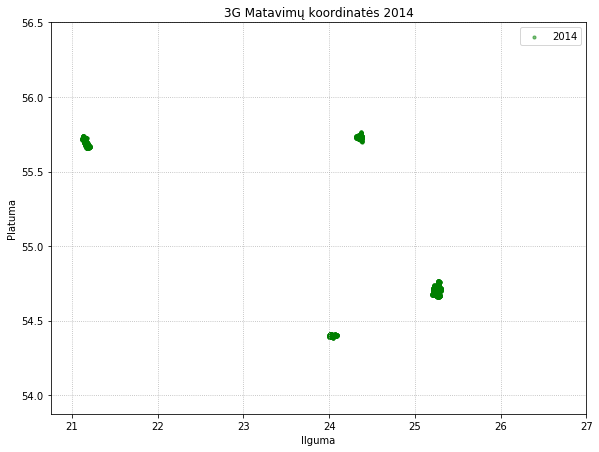
\includegraphics[scale=0.33]{img/3G-1}
	\caption{3G Matavimai 2014 metais. Viso – 2245 matavimai.}
	\label{img:3G-1}
\end{figure}
\begin{figure}[H]
	\centering
	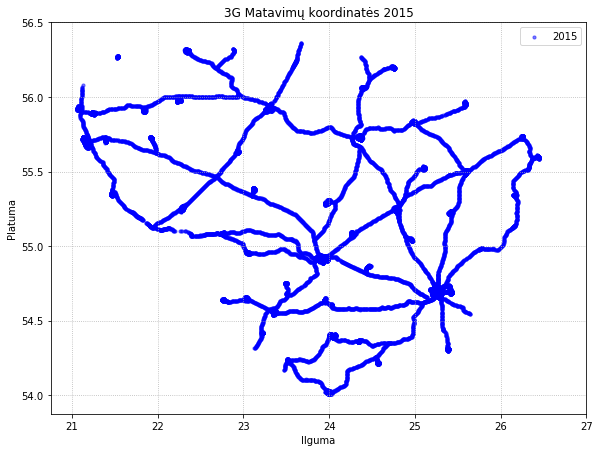
\includegraphics[scale=0.33]{img/3G-2}
	\caption{3G Matavimai 2015 metais. Viso – 19427 matavimai.}
	\label{img:3G-2}
\end{figure}
\begin{figure}[H]
	\centering
	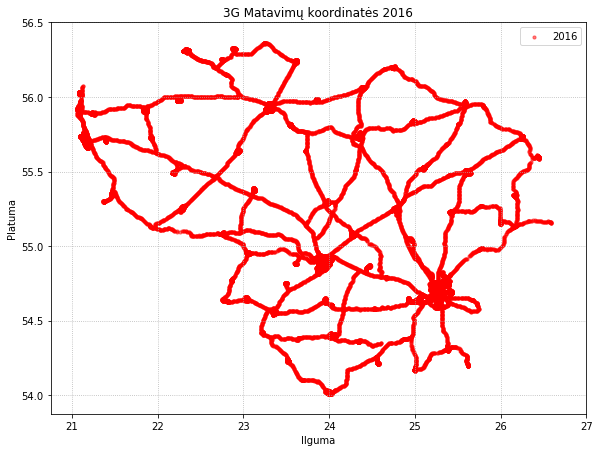
\includegraphics[scale=0.33]{img/3G-3}
	\caption{3G Matavimai 2016 metais. Viso – 34769 matavimai.}
	\label{img:3G-3}
\end{figure}
\begin{figure}[H]
	\centering
	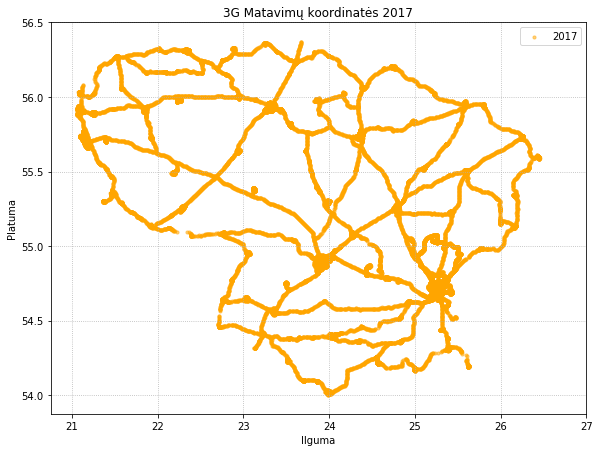
\includegraphics[scale=0.33]{img/3G-4}
	\caption{3G Matavimai 2017 metais. Viso – 38789 matavimai.}
	\label{img:3G-4}
\end{figure}
\begin{figure}[H]
	\centering
	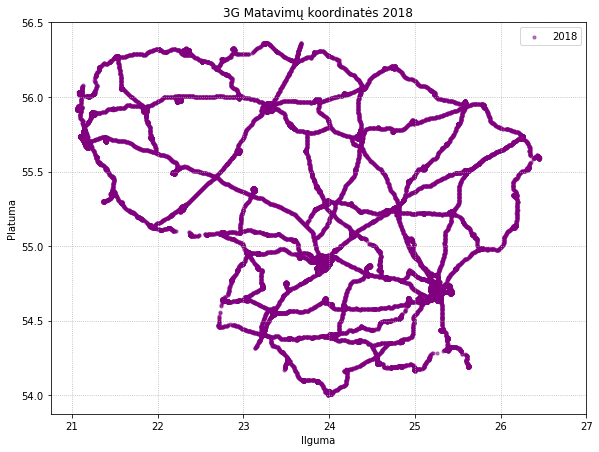
\includegraphics[scale=0.33]{img/3G-5}
	\caption{3G Matavimai 2018 metais. Viso – 40773 matavimai.}
	\label{img:3G-5}
\end{figure}
IPSS LTE ryšio technologijos matavimai 2014–2018 metais. Viso 157522 įrašai.
\begin{figure}[H]
	\centering
	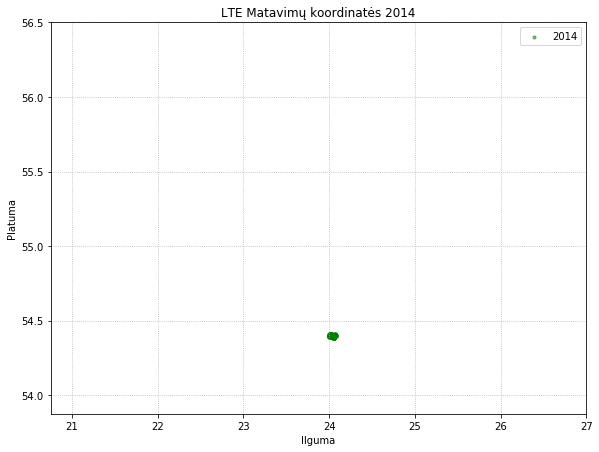
\includegraphics[scale=0.33]{img/LTE-1}
	\caption{LTE Matavimai 2014 metais. Viso – 232 matavimai.}
	\label{img:LTE-1}
\end{figure}
\begin{figure}[H]
	\centering
	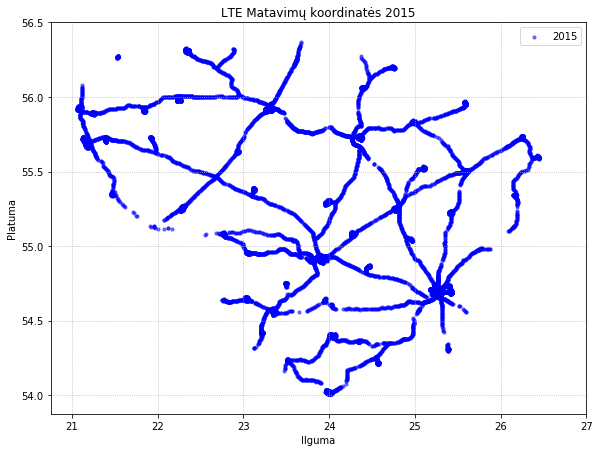
\includegraphics[scale=0.33]{img/LTE-2}
	\caption{LTE Matavimai 2015 metais. Viso – 13962 matavimai.}
	\label{img:LTE-2}
\end{figure}
\begin{figure}[H]
	\centering
	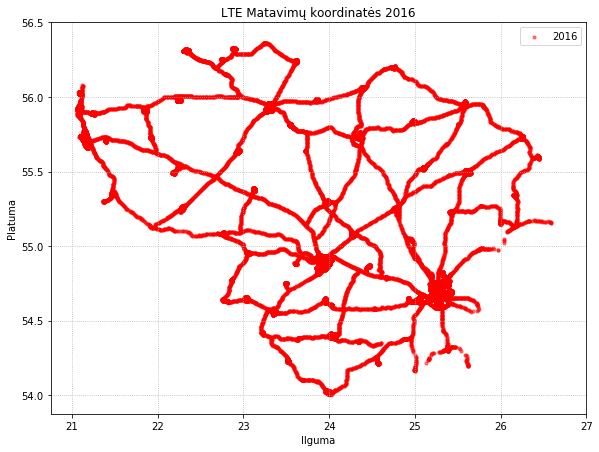
\includegraphics[scale=0.33]{img/LTE-3}
	\caption{LTE Matavimai 2016 metais. Viso – 40738 matavimai.}
	\label{img:LTE-3}
\end{figure}
\begin{figure}[H]
	\centering
	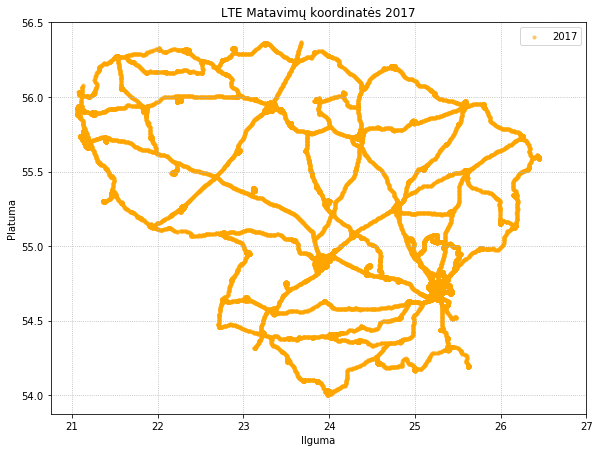
\includegraphics[scale=0.33]{img/LTE-4}
	\caption{LTE Matavimai 2017 metais. Viso – 49672 matavimai.}
	\label{img:LTE-4}
\end{figure}
\begin{figure}[H]
	\centering
	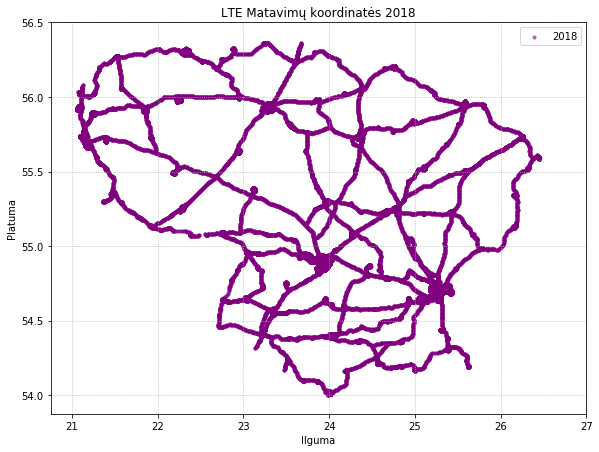
\includegraphics[scale=0.33]{img/LTE-5}
	\caption{LTE Matavimai 2018 metais. Viso – 52918 matavimai.}
	\label{img:LTE-5}
\end{figure}
IPSS WiMAX ryšio technologijos matavimai 2014–2018 metais. Viso 18166 įrašai.
\begin{figure}[H]
	\centering
	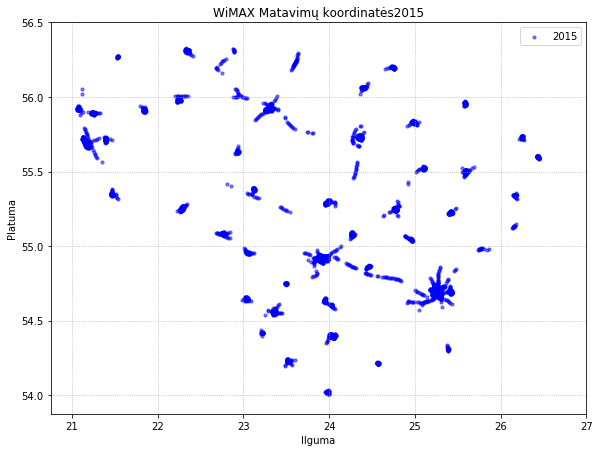
\includegraphics[scale=0.33]{img/WiMAX-1}
	\caption{WiMAX Matavimai 2015 metais. Viso – 4307 matavimai.}
	\label{img:WiMAX-1}
\end{figure}
\begin{figure}[H]
	\centering
	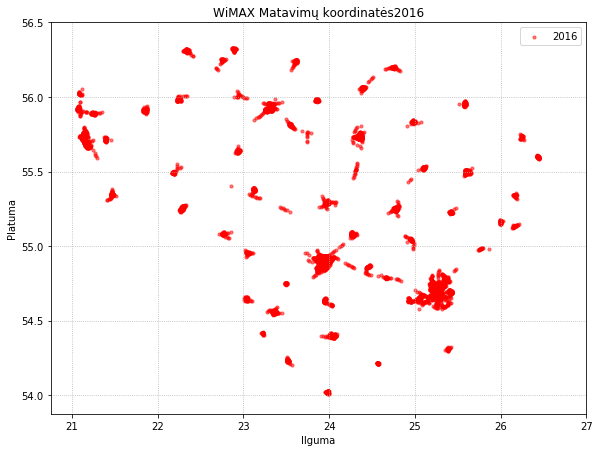
\includegraphics[scale=0.33]{img/WiMAX-2}
	\caption{WiMAX Matavimai 2016 metais. Viso – 7653 matavimai.}
	\label{img:WiMAX-2}
\end{figure}
\begin{figure}[H]
	\centering
	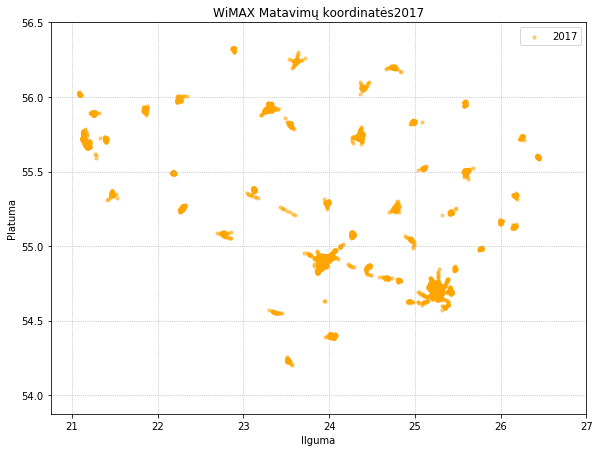
\includegraphics[scale=0.33]{img/WiMAX-3}
	\caption{WiMAX Matavimai 2017 metais. Viso – 6206 matavimai.}
	\label{img:WiMAX-3}
\end{figure}

\section{Pradinių IPSS CSV failų apdorojimo „Python“ skriptas} \label{script1}
„Python“ skriptas skirtas iš duotųjų IPSS duomenų CSV failų atrinkti nereikalingus laukus ir pervadinti lietuviškus antraštės pavadinimus į vieno žodžio (vienos simbolių eilutės) angliškus pavadinimus bei sugeneruoti naujus CSV failus:
\lstinputlisting[language=Python]{scripts/script1.py}

\section{Atrinktų IPSS CSV failų duomenų papildymo „Python“ skriptas} \label{script2}
„Python“ skriptas skirtas jau atrinktiems CSV failams pridėti papildomus laukus: aukščio virš jūros lygio (gaunamas iš koordinačių), suapvalintų koordinačių reikšmių bei suapvalintos aukščio reikšmės. Šiems duomenims yra sugeneruojamas nauji CSV failai:
\lstinputlisting[language=Python]{scripts/script2.py}



\section{Eksperimentinio palyginimo rezultatai}
% tablesgenerator.com - converts calculators (e.g. excel) tables to LaTeX
\begin{table}[H]\footnotesize
	\centering
	\caption{Lentelės pavyzdys}
	{\begin{tabular}{|l|c|c|} \hline
			Algoritmas & $\bar{x}$ & $\sigma^{2}$ \\
			\hline
			Algoritmas A  & 1.6335    & 0.5584       \\
			Algoritmas B  & 1.7395    & 0.5647       \\
			\hline
	\end{tabular}}
	\label{tab:table example}
\end{table}

\end{document}

			Algoritmas & $\bar{x}$ & $\sigma^{2}$ \\
			\hline
			Algoritmas A  & 1.6335    & 0.5584       \\
			Algoritmas B  & 1.7395    & 0.5647       \\
			\hline
	\end{tabular}}
	\label{tab:table example}
\end{table}

\end{document}
